\documentclass{beamer}
\setbeamertemplate{navigation symbols}{}

\usepackage{tikz}
\usepackage{listings}

\usetheme{Warsaw}

\beamersetuncovermixins{\opaqueness<1>{25}}{\opaqueness<2->{15}}
\begin{document}
\title{LexBFS and its applications}  
\author{Guillaume Aubian}
\date{\today} 


\begin{frame}
\titlepage
\end{frame}

\begin{frame}\frametitle{Overview}\tableofcontents
\end{frame} 


\section{Graph Searches} 
\begin{frame}\frametitle{What's in a graph ?}
    \begin{block}{Graph}
	We consider non-oriented, simple and \textbf{connected} graphs
    \end{block}
    INCLUDE GRAPHS EXAMPLES AND COUNTEREXAMPLES
\end{frame}

\begin{frame}[fragile]\frametitle{Generic Search}
    \begin{lstlisting}[language = Python]
    for i in [1, ..., n]:
        if i == 1:
	    u = any vertex
	else:
	    u = any unvisited marked vertex
	visit(u)
	for v in neighbours(u):
	    mark(v)
    \end{lstlisting}
\end{frame}

\begin{frame}\frametitle{Another Characterization}
    Let's number vertices in the order they are visited.
    \begin{theorem}
        An order $\sigma$ corresponds to a Generic Search if and only if
	    
	    $$\forall a <_{\sigma} b <_{\sigma} c, ac \in E\text{ and }ab \notin E, \exists d <_{\sigma} b\text{ st }db \in E$$
    \end{theorem}
    \begin{center}
    \begin{tikzpicture}
	\draw (0,1) arc (120:60:4) ;
	\draw [dashed] (0,1) -- (2,1);
	\draw (0,0) -- (2,1);
	\draw (0,0) node[below]{$d$} ;
	\draw (0,1) node[below]{$a$} ;
	\draw (2,1) node[below]{$b$} ;
	\draw (4,1) node[below]{$c$} ;
	\draw [dotted] (1,-0.5) -- (1,1.5);
	\draw [dotted] (3,-0.5) -- (3,1.5);
	\draw (1,-0.5) node[below]{$<$} ;
	\draw (3,-0.5) node[below]{$<$} ;
    \end{tikzpicture}
    \end{center}
\end{frame}

\begin{frame}[fragile]\frametitle{DFS}
    INCLUDE GRAPH EXAMPLE
    \begin{lstlisting}[language = Python]
    for i in [1, ..., n]:
        if i == 1:
	    u = any vertex
	else:
	    u = any unvisited vertex w/ max label
	visit(u)
	for v in neighbours(u):
	    label[v] = i
    \end{lstlisting}
\end{frame}

\begin{frame}\frametitle{Another Characterization}
    \begin{theorem}
        An order $\sigma$ corresponds to a DFS if and only if
	    
	    $$\forall a <_{\sigma} b <_{\sigma} c, ac \in E\text{ and }ab \notin E, \exists a <_{\sigma} d <_{\sigma} b\text{ st }db \in E$$
    \end{theorem}
    \begin{center}
    \begin{tikzpicture}
	\draw (0,0) arc (120:60:6) ;
	\draw (2,0) -- (4,0);
	\draw [dashed] (0,0) arc (120:60:4) ;

	\draw (0,0) node[below]{$a$} ;
	\draw (2,0) node[below]{$d$} ;
	\draw (4,0) node[below]{$b$} ;
	\draw (6,0) node[below]{$c$} ;

	\draw [dotted] (1,-0.5) -- (1,1.5);
	\draw [dotted] (3,-0.5) -- (3,1.5);
	\draw [dotted] (5,-0.5) -- (5,1.5);

	\draw (1,-0.5) node[below]{$<$} ;
	\draw (3,-0.5) node[below]{$<$} ;
	\draw (5,-0.5) node[below]{$<$} ;
    \end{tikzpicture}
    \end{center}

\end{frame}


\begin{frame}[fragile]\frametitle{BFS}
    \begin{lstlisting}[language = Python]
    for i in [n, ..., 1]:
        if i == n:
	    u = any vertex
	else:
	    u = any unvisited vertex w/ max label
	visit(u)
	for v in neighbours(u):
	    if v has no label:
	        label[v] = i
    \end{lstlisting}


    INCLUDE GRAPH EXAMPLE
\end{frame}

\begin{frame}\frametitle{Another Characterization}
    \begin{theorem}
        An order $\sigma$ corresponds to a BFS if and only if
	    
	    $$\forall a <_{\sigma} b <_{\sigma} c, ac \in E\text{ and }ab \notin E, \exists d <_{\sigma} a\text{ st }db \in E$$
    \end{theorem}

    \begin{center}
    \begin{tikzpicture}
	\draw (0,0) arc (120:60:4) ;
	\draw (2,0) arc (120:60:4) ;
	\draw [dashed] (2,0) -- (4,0);

	\draw (0,0) node[below]{$d$} ;
	\draw (2,0) node[below]{$a$} ;
	\draw (4,0) node[below]{$b$} ;
	\draw (6,0) node[below]{$c$} ;

	\draw [dotted] (1,-0.5) -- (1,1.5);
	\draw [dotted] (3,-0.5) -- (3,1.5);
	\draw [dotted] (5,-0.5) -- (5,1.5);

	\draw (1,-0.5) node[below]{$<$} ;
	\draw (3,-0.5) node[below]{$<$} ;
	\draw (5,-0.5) node[below]{$<$} ;
    \end{tikzpicture}
    \end{center}

\end{frame}

\begin{frame}[fragile]\frametitle{Let's rewrite BFS}

    \begin{lstlisting}[language = Python]
    for i in [n, ..., 1]:
        if i == n:
	    u = any vertex
	else:
	    u = any unvisited vertex
	        w/ max first element of label
	visit(u)
	for v in neighbours(u):
	    label[v].append(i)
    \end{lstlisting}

    INCLUDE GRAPH EXAMPLE
\end{frame}

\begin{frame}[fragile]\frametitle{Here is LexBFS}
    \begin{lstlisting}[language = Python]
    for i in [n, ..., 1]:
        if i == n:
	    u = any vertex
	else:
	    u = any unvisited vertex
	        w/ max lexicographical label
	visit(u)
	for v in neighbours(u):
	    label[v].append(i)
    \end{lstlisting}

	
    INCLUDE GRAPH EXAMPLE
\end{frame}

\begin{frame}\frametitle{Another Characterization}
    \begin{theorem}
        An order $\sigma$ corresponds to a LexBFS if and only if
	    
	    $$\forall a <_{\sigma} b <_{\sigma} c, ac \in E\text{ and }ab \notin E, \exists d <_{\sigma} a\text{ st }db \in E\text{ and }dc \notin E$$
    \end{theorem}

    \begin{center}
    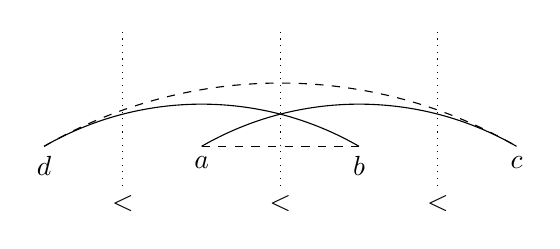
\begin{tikzpicture}
	\draw (0,0) arc (120:60:4) ;
	\draw (2,0) arc (120:60:4) ;
	\draw [dashed] (2,0) -- (4,0);
	\draw [dashed] (0,0) arc (120:60:6) ;

	\draw (0,0) node[below]{$d$} ;
	\draw (2,0) node[below]{$a$} ;
	\draw (4,0) node[below]{$b$} ;
	\draw (6,0) node[below]{$c$} ;

	\draw [dotted] (1,-0.5) -- (1,1.5);
	\draw [dotted] (3,-0.5) -- (3,1.5);
	\draw [dotted] (5,-0.5) -- (5,1.5);

	\draw (1,-0.5) node[below]{$<$} ;
	\draw (3,-0.5) node[below]{$<$} ;
	\draw (5,-0.5) node[below]{$<$} ;
    \end{tikzpicture}
    \end{center}
\end{frame}

\end{document}
